\section{Model-agnostic methods}
Separating the explanations from the machine learning model (= model-agnostic interpretation methods) has some advantages:
\begin{itemize}
    \item \textbf{Model Flexibility}: The interpretation method can work with any machine learning model, including interpretable ones such as random forests and deep neural networks.
    \item \textbf{Explanation flexibility:} You are not limited to a certain form of explanation. In some case it might be useful to have a linear formula, in other cases a graphic with feature importance.
    \item \textbf{Representation flexibility:} The explanation system should be able to use a different feature representation as the model being explained.
\end{itemize}

\subsection{Permutation Feature Importance}
The importance of a feature is the increase in the prediction error of the model after we permuted the feature's values, which breaks the relationship between the feature and the true outcome.
The permutation feature importance algorithm based on Fisher, Rudin, and Dominici (2018):\\

Input: Trained model $f$, feature matrix $X$\, target vector $y$, error measure $L(y, f)$\\
\begin{enumerate}
    \item Esitmate the original model error $e^{orig}=L(y, f(X))$ (e.g mean squared error)
    \item For each feature $j=1\ldots p$ do:
    \begin{itemize}
        \item Generate a permuted feature matrix $X_{permuted}$ by shuffling the values in the $j$-th column of $X$. This breaks the association between the feature and the target.
        \item Esitmate the error of the model on the permuted feature matrix $e^{perm}=L(y, f(X_{permuted}))$
        \item Calculate the feature importance as the difference between the original error and the permuted error $FI^j=e^{perm}-e^{orig}$ or $FI^j=\frac{e^{perm}}{e^{orig}}$
    \end{itemize}
    \item Sort the feature importance values $FI^j$ in descending order.
\end{enumerate}

\subsubsection{Feature importance \- Training or Test data?}
\begin{itemize}
    \item Feature importance based on the training data tells us which features are important for the model in the sense that it depends on them for making predictions.
    \item Feature importance based on unseen (test) data talks about the generalization properties of the trained final model.
\end{itemize}

In the end, you need to decide whether you want to know \textbf{how much the model relies on each feature for making predictions (-> training data)} or \textbf{how much the feature contributes to the performance of the model on unseen data (-> test data)}.

\subsection{Global surrogate model}
A global surrogate model is an interpretable model that is trained to approximate the predictions of a black box model. We can draw conclusions about the black box model by interpreting the surrogate model.
We want to approximate our black box prediction function $f$ as closely as possible with the surrogate model prediction function $g$, under the constraint that $g$ is interpretable.
The surrogate model is agnostic as it only requires to know the predictions of the black box model.

\subsubsection{Global surrogate model recipe}
\begin{enumerate}
    \item Select a dataset $X$: This can be the same dataset that was used for training the black box model or a new dataset from
    the same distribution. You could even select a subset of the data or a grid of points, depending on
    your application
    \item Get the predictions of the black box model $f$ on the dataset $X$: $f(X)$
    \item Select an interpretable model type (linear model, decision tree, …).
    \item Train the interpretable model on the dataset $X$ with the predictions of the black box model as the target variable.
    \item Measure the performance of the surrogate model: Compare the predictions of the surrogate model with the predictions of the black box model on a test set.
    \item Interpret the surrogate model: Use the interpretable model to draw conclusions about the black box model.
\end{enumerate}

You may find approaches for surrogate models that have some extra steps or differ a little, but the general idea is usually as described here.
One way to measure how well the surrogate replicates the black box model is the R-squared measure:
\begin{equation*}
    R^2=1-\frac{SSE}{SST}=1-\frac{\sum_{i=1}^n(\hat{y}_*^{(i)}-\hat{y}^{(i)})^2}{\sum_{i=1}^n(\hat{y}^{(i)}-\bar{\hat{y}})^2}
\end{equation*}
where $\hat{y}_*^{(i)}$ are the predictions of the surrogate model, $\hat{y}^{(i)}$ are the predictions of the black box model, and $\bar{\hat{y}}$ is the mean of the black box model predictions.
SSE stands for sum of squares error and SST for sum of squares total.

The R-squared measure can be interpreted as the percentage of variance that is captured by the surrogate model.
\begin{itemize}
    \item If R-squared is close to 1 (= low SSE), then the interpretable model approximates the behavior of
    the black box model very well. If the interpretable model is very close, you might want to replace the
    complex model with the interpretable model.
    \item If the R-squared is close to 0 (= high SSE), then the interpretable model fails to explain the black box model.
\end{itemize}

\subsubsection{Towards Local Surrogate Models}
We could also build a surrogate model based on a subset of the original data or reweight the instances.
In this way, we change the distribution of the surrogate model's input, which changes the focus of the interpretation (then it is no longer really global).

If we weight the data locally by a specific instance of the data (the closer the instances to the selected instance, the higher their weight), we get a local surrogate model that can explain the individual prediction of the instance.

\subsection{Local Interpretable Model-agnostic Explanation (LIME)}
Local surrogate models are interpretable models that are used to explain individual predictions of black box machine learning models.
Instead of training a global surrogate model, LIME focuses on training local surrogate models to explain individual predictions
It does not have to be able to reproduce the black box model predictions overall, but only locally $\rightarrow$ local fidelity.\\

The idea is quite intuitive. First, forget about the training data and imagine you only have the black box model where you can input data points and get the predictions of the model. 
You can probe the box as often as you want. Your goal is to understand why the machine learning model made a certain prediction. LIME tests what happens to the predictions when you give variations of your data into the machine learning model. 
LIME generates a new dataset consisting of perturbed samples and the corresponding predictions of the black box model. On this new dataset LIME then trains an interpretable model, which is weighted by the proximity of the sampled instances to the instance of interest.

Local surrogate models with interpretability constraints can be formalized as follows:
\begin{equation*}
    \text{explanation}(x)=\arg\min_{g\in{}G}L(f,g,\pi_x)+\Omega(g)
\end{equation*}
The explanation model for the instance $x$ is the model $g$ that minimizes the loss $L$ which measures how well the explanation model approximates the prediction of the original model $f$, while the model complexity $\Omega(g)$ is kept low.
The proximity defines how large the neighborhood around instance $x$ is that we consider for the explanation (kernel).

In practice, LIME only optimizes the loss part. The user has to determine the complexity.

\subsubsection{LIME Algorithm}
\begin{enumerate}
    \item Select the instance to be explained $x$
    \item Generate points all over the $\mathbb{R}^p$ space (sample $N$ values from a normal distribution inferred from the training set)
    \item Weight the new samples according to their proximity to the instance of interest. (e.g.\ using RBF kernel which assigns higher weights to points closer to the reference)
    \item Get the predictions of the black box model for the perturbed samples
    \item Train a weighted, interpretable model on the perturbed samples with the predictions of the black box model as the target variable
    \item Explain the prediction by interpreting the local model
\end{enumerate}
The coefficients obtained from such explainable models represent the LIME values. Comparing the coefficients of the explainable model assigned to each input variable it is
possible to understand which variables are the most relevant for the selected instance $x_i$

\subsubsection{General intuition}
By training a complex ML model we obtain a complex and wiggly prediciton curve $f(x)$. LIME's goal is to find its tangent at a precise point (reference point).
From Taylor Theorem we know that each function can be approximated using polynomials (the higher the degree, the lower the approximation error).
The tangent is the Taylor polynomial of degree 1, since the degree is low, to obtain a good approximation we should consider a small region around the reference.\\

If the $f(x)$ is analytically known it would have just been sufficient to calculate its derivative analytically. However since we are considering ML derived $f(x)$ we do not know the formula hence we can't calculate the derivative.

\subsubsection{LIME advantages}
\begin{itemize}
    \item Even if you replace the underlying machine learning model, you can still use the same local, interpretable model for explanations.
    \item It works for tabular data, text and images.
    \item The fidelity measure (how well the interpretable model approximates the black box predictions) gives us a good idea of how reliable
    the interpretable model is in explaining the black box predictions in the neighborhood of the data instance of interest
\end{itemize}

\subsubsection{LIME disadvantages}
\begin{itemize}
    \item The correct definition of the neighborhood is a very big, unsolved problem when using LIME with tabular data.
    \item Sampling could be improved in the current implementation of LIME. Data points are sampled from a Gaussian distribution inferred from the training data, ignoring the correlation across features.
    \item The complexity of the explanation model (e.g. K. number of features to be used) has to be defined in advance
    \item Instability of the explanations (i.e close points can lead to very different explanations, as well as different sampling instances). This leads to low trustflulness of the explanations.
\end{itemize}

\subsection{SHapley Additive exPlanation \- SHAP}
SHAP by Lundberg and Lee (2017)\cite{Lundberg2017} is a method to explain individual predictions (local agnostic).
Explains the prediction of an instance $x$ as a sum of contributions from individual feature values.
The SHAP explanation method computes Shapley values from coalitional game theory. The feature values of a data instance act as players in a coalition. Shapley values tell us how to fairly distribute the “payout” (= the prediction) among the features.
\subsubsection{Shapley values}
The Shapley value is a method for assigning payouts to players depending on their contribution to the total payout. Players cooperate in a coalition and receive a certain profit from this cooperation..
In the context of Machine Learning, the Game is the prediction task for a single instance in the dataset. The Gain is the actual prediction for this instance minus the average prediction for all instances. The Players are the feature values of the instances that collaborate to receive the gain (predict a certain value).\\

The Shapley value is the average marginal contribution of a feature value across all possible coalitions (i.e combination of features).
To obtain the contribution of each player (feature) in the game (model) it is required to train a distinct predictive model for each distinct coalition in the power set, meaning $2^F$ models.
Once we trained all the models, we can then take a new observation (let us call it $x_0$) and see what the different models predict for the same observation $x_0$.
The difference between the prediction of the model with the feature $i$ and the model without the feature $i$ is the marginal contribution of the feature $i$ to the prediction of the observation $x_0$.
The Shapley value is the (weighted) average of marginal contributions across coalitions.\\

To obtain the prediction in all models, we replace the feature values of the features that are not in a coalition with random feature values from the corresponding set to get a prediction from the machine learning model.

\textbf{General formulation:}
Generalizing for any feature $x$ and number of features $F$
\begin{equation*}
    SHAP_{feature}(x)=\sum_{set:feature\in{}set}{[|set|\times\binom{F}{|set|}]}^{-1}[Predict_{set}(x)-Predict_{set\backslash{}feature}(x)]
\end{equation*}

\textbf{Shapley values \ Properties}
The Shapley value is the only attribution method that satisfies the properties Efficiency, Symmetry, Dummy and Additivity, which together can be considered a definition of a fair payout.
\begin{itemize}
    \item \textbf{Efficiency:} The sum of the Shapley values equals the difference between the prediction for the instance and the average prediction for all instances.
    \item \textbf{Symmetry:} If two players have the same impact on the payout in all coalitions, they should receive the same Shapley value.
    \item \textbf{Dummy:} If a player does not change the payout in any coalition, its Shapley value should be zero.
    \item \textbf{Additivity:} The Shapley value of the sum of two players should be the sum of the Shapley values of the two players.
\end{itemize}

\subsubsection{SHAP \- LIME connection}
Shapley value explanation is represented as an additive feature attribution method, a linear model. That view connects LIME and Shapley values. SHAP specifies the explanation as:ù
\begin{equation*}
    g(z')=\phi_0+\sum_{j=1}^M\phi_jz_j'
\end{equation*}
Where $g$ is the explanation mode, $z'\in\{0,1\}^M$ is the coalition vector, $M$ is the maximum coalition size and $\phi_j\in\mathbb{R}$ is the feature attribution for a feature $j$, the Shapley values.
In the coalition vector an entry of 1 means the corresponding feature is present and 0 that is absent.

For $x$ the instance to be explained, the coalition vector $z'$ is a vector of all 1. The formula becomes:
\begin{equation*}
    g(x')=\sum_{j=1}^M\phi_j
\end{equation*}

\subsubsection{SHAP properties revisited}
SHAP satisfies all the properties of efficiency, symmetry, dummy and additivity as the Shapley value since it computes them.
Moreover, SHAP follows also three desirable properties:
\begin{itemize}
    \item \textbf{Local accuracy:} The explanation model is accurate in the neighborhood of the instance to be explained.
    \item \textbf{Missingness:} If a feature is missing, the corresponding Shapley value is zero.
    \item \textbf{Consistency:} If the model is changed in a way that does not affect the prediction, the Shapley values should not change.
\end{itemize}

\subsection{Approximate SHAP values}
The exact computation of Shapley values is computationally infeasible for most machine learning models. The number of coalitions grows exponentially with the number of features. Hence we need to approximate the Shapley values.\\

\textbf{Kernel SHAP}
ss a method that uses the LIME framework to compute Shapley Values. Setting the loss function, weighting kernel and regularization terms appropriately in the LIME framework allows theoretically obtaining Shapley Values more efficiently than directly computing Shapley Values.
The Kernel SHAP algorithm is as follows:
\begin{enumerate}
    \item Sample coalitions $z_k'\in\{0,1\}^M,\quad{}k\in\{1,\ldots,K\}$ (1 = feature present in coalition, 0 = feature absent).
    \item Get prediction for each $z_k'$ by first converting $z_k'$  to the original feature space and then applying model $\hat{f}: \hat{f}(h_x(z_k'))$.
    \item Compute the weight for each $z_k'$ using the SHAP kernel.
    \item Fit weighted linear model.
    \item Return Shapley values $\phi_k$,the coefficients from the linear model.
\end{enumerate}
Difference between LIME and KernelSHAP:\\
The big difference to LIME is the weighting of the instances in the regression model.
\begin{itemize}
    \item LIME weights the instances according to how close they are to the original instance. The more 0's in the coalition vector, the smaller the weight in LIME.
    \item KernelSHAP weights the sampled instances according to the weight the coalition would get in the Shapley value estimation.\\
\end{itemize}

\textbf{TreeSHAP}
Lundberg et al. proposed TreeSHAP, a variant of SHAP for tree-based machine learning models such as decision trees, random forests and gradient boosted trees. TreeSHAP was introduced as a fast, model-specific alternative to KernelSHAP, but it turned out that it can produce unintuitive feature attributions.

TreeSHAP defines the value function using the conditional expectation $E_{X_j|X_{-j}}(\hat{f}(x)|x_j)$ instead of the marginal expectation.
The problem with the conditional expectation is that features that have no influence on the prediction function f can get a TreeSHAP estimate different from zero as shown by \cite{Mukund2019shanpley}.
The non-zero estimate can happen when the feature is correlated with another feature that actually has an influence on the prediction.

\subsection{SHAP feature importance}
To obtain global information it is possible to average the absolute Shapley values per feature across the data.

\subsection{SHAP Summary Plot}
\begin{figure}[H]
    \centering
    \begin{minipage}{0.40\textwidth}
        The summary plot combines feature importance with feature effects. Each point on the summary plot is a Shapley value for a feature and an instance. The position on the y-axis is determined by the feature and on the x-axis by the Shapley value. The color represents the value of the feature from low to high. Overlapping points are jittered in y-axis direction, so we get a sense of the distribution of the Shapley values per feature. The features are ordered according to their importance.\\

        In the summary plot, we see first indications of the relationship between the value of a feature and the impact on the prediction. But to see the exact form of the relationship, we have to look at SHAP dependence plots.
    \end{minipage}
    \hfill
    \begin{minipage}{0.55\textwidth}
        \begin{figure}[H]
            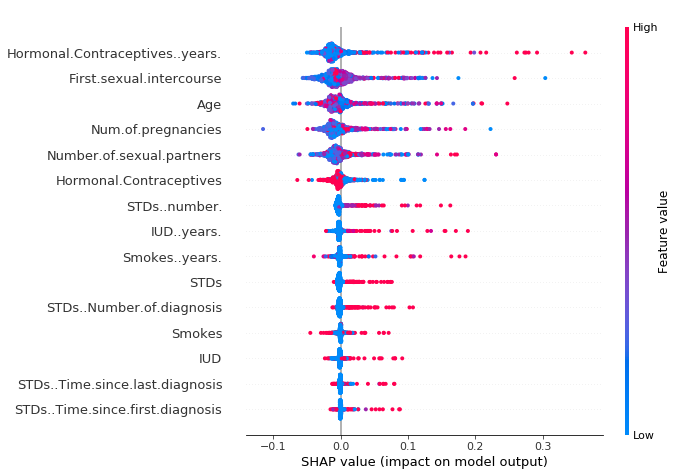
\includegraphics[width=\textwidth]{img/shap-importance-extended.png}
            \centering
        \end{figure}
    \end{minipage}
\end{figure}

\subsection{SHAP Dependence Plot}
\begin{figure}[H]
    \centering
    \begin{minipage}{0.40\textwidth}
        SHAP feature dependence might be the simplest global interpretation plot:
        \begin{enumerate}
            \item Pick a feature
            \item For each data instance, plot a point with the feature value on the x-axis and the corresponding Shapley value on the y-axis.
            \item Done\\
        \end{enumerate}

        Mathematically, the plot contains the following points: $\{(x_j^{(i)},\phi_j^{(i)})\}_{i=1}^n$\\

        SHAP dependence plots are an alternative to partial dependence plots and accumulated local effects. While PDP and ALE plot show average effects, SHAP dependence also shows the variance on the y-axis. Especially in case of interactions, the SHAP dependence plot will be much more dispersed in the y-axis. The dependence plot can be improved by highlighting these feature interactions.
    \end{minipage}
    \hfill
    \begin{minipage}{0.55\textwidth}
        \begin{figure}[H]
            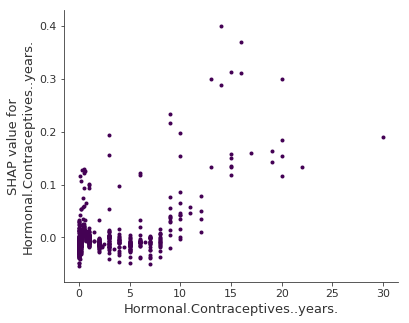
\includegraphics[width=\textwidth]{img/shap-dependence.png}
            \centering
        \end{figure}
    \end{minipage}
\end{figure}
\newpage
\subsection{Clustering Shapley Values}
You can cluster your data with the help of Shapley values. The goal of clustering is to find groups of similar instances. Normally, clustering is based on features. Features are often on different scales. For example, height might be measured in meters, color intensity from 0 to 100 and some sensor output between -1 and 1. The difficulty is to compute distances between instances with such different, non-comparable features.

SHAP clustering works by clustering the Shapley values of each instance. This means that you cluster instances by explanation similarity.
All SHAP values have the same unit – the unit of the prediction space. You can use any clustering method.
\begin{figure}[H]
    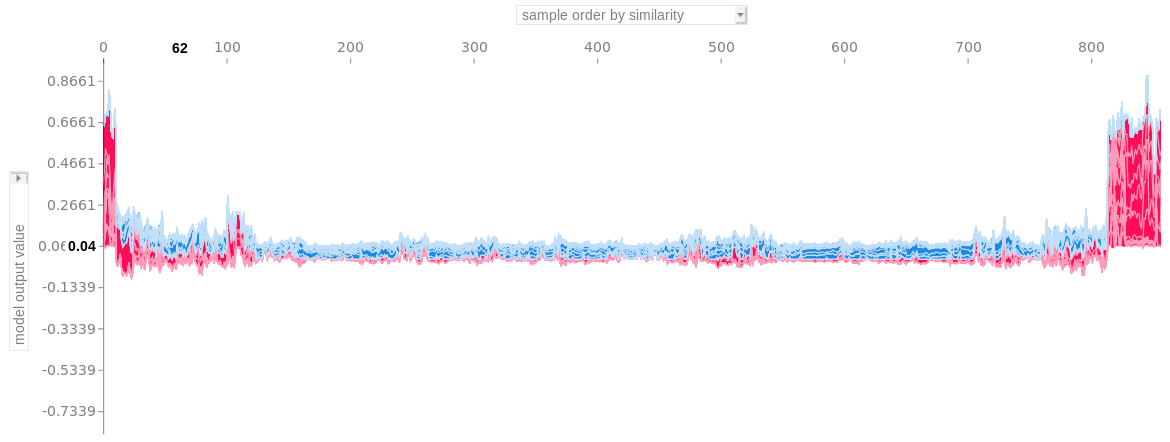
\includegraphics[width=0.8\textwidth]{img/shap-clustering.png}
    \centering
\end{figure}

\subsection{Advatages/Disadvantages}
\textbf{Advantages:}\\
\begin{itemize}
    \item SHAP has a solid theoretical foundation in game theory.
    \item The prediction is fairly distributed among the feature values. We get contrastive explanations that compare the prediction with the average prediction.
    \item We get contrastive explanations that compare the prediction with the average prediction.
\end{itemize}
\textbf{Disadvantages:}\\
\begin{itemize}
    \item KernelSHAP is slow. This makes KernelSHAP impractical to use when you want to compute Shapley values for many instances. Also, all global SHAP methods such as SHAP feature importance require computing Shapley values for a lot of instances.
    \item KernelSHAP ignores feature dependence. Most other permutation-based interpretation methods have this problem. By replacing feature values
    with values from random instances, it is usually easier to randomly sample from the marginal
    distribution. However, if features are dependent, e.g. correlated, this leads to putting too much weight
    on unlikely data points.
\end{itemize}